\chapter{Antecedentes}
En este capítulo se presentan los antecedentes y conceptos teóricos necesarios para entender este trabajo.
\section{Control de flujo de información}
Los lenguajes con tipado de seguridad para el control del flujo de la información clasifican los valores de un programa con respecto a sus niveles de confidencialidad, expresado mediante una \emph{lattice}\footnote{Un orden parcial, donde todo par de elementos tiene un único supremo e ínfimo} de etiquetas de seguridad. Por ejemplo, con la lattice de dos niveles de seguridad \texttt{L} $\sqsubseteq$ \texttt{H} se puede distinguir entre valores públicos o de baja confidencialidad (\texttt{L}) y valores privados o de alta confidencialidad (\texttt{H}). Un sistema de tipos con control de flujo asegura de forma estática el cumplimiento de la propiedad \emph{noninterference}~\cite{noninterference}, esto es, que la información confidencial no fluya directa o indirectamente hacia canales públicos~\cite{volpanoAl:S96}.

En el siguiente ejemplo se muestra un código anotado con niveles de seguridad, en donde el parámetro \texttt{guess} y el retorno del método se declaran de baja confidencialidad, y el parámetro \texttt{password} se declara de alta confidencialidad. Además, se considera que los valores literales son de baja confidencialidad.

\begin{ej} \ \\
  \normalfont
  \label{ej2-1}
\begin{lstlisting}
  String@L login(String@L guess, String@H password) {
    if (password == guess) return "Login successful";
    else return "Login failed";
  }
\end{lstlisting}
\end{ej}

En el ejemplo \ref{ej2-1} ocurrió un \emph{flujo explícito}, debido a que un observador público puede obtener información del parámetro confidencial \texttt{password} observando las salidas del programa. Si en cambio el método \texttt{login} declara un retorno de tipo \texttt{String@H}, un observador público no podrá leer la salida del programa, por lo que no ocurre un flujo explícito.

En el siguiente ejemplo se introduce una variable global al ejemplo \ref{ej2-1} para almacenar el valor de retorno, y se cambia el tipo de retorno de la función por \texttt{void}.

\begin{ej} \ \\
  \normalfont
  \label{ej2-12}
\begin{lstlisting}
  String@L ret = "";
  void login(String@L guess, String@H password) {
    if (password == guess) ret = "Login successful";
    else ret = "Login failed";
  }
\end{lstlisting}
\end{ej}

En el ejemplo \ref{ej2-12} ocurrió un \emph{flujo implícito}, debido a que un observador público puede obtener información del parámetro confidencial \texttt{password} observando cambios en el bloque de memoria que almacena el valor de la variable \texttt{ret}.

La ocurrencia de flujos explícitos e implícitos significa una infracción a noninterference. En los ejemplos \ref{ej2-1} y \ref{ej2-12}, es posible detectar estos flujos considerando que las instrucciones de retorno y asignación de valores de baja confidencialidad, ocurren en un contexto de alta confidencialidad, determinado por la condición de la instrucción \texttt{if}. Para considerar el contexto de ejecución de una instrucción en las reglas del sistema de tipos, se utiliza el concepto de \textit{program counter} (\texttt{pc}) para seguridad~\cite{pc}. Así, en los ejemplos \ref{ej2-1} y \ref{ej2-12} las instrucciones de retorno y asignación son inválidas, debido a que retornan y asignan valores de baja confidencialidad cuando el \texttt{pc} tiene un valor de alta confidencialidad.

A pesar de que noninterference es una propiedad atractiva para la especificación de sistemas seguros, se considera muy estricta en la práctica, debido a que impide que la información confidencial tenga cualquier tipo de influencia en una salida observable de un programa. En efecto, queremos que el programa de \texttt{login} sea aceptado a pesar de infringir noninterference, pues de otra forma no tendríamos cómo realizar la autenticación.

Para solucionar este problema, los lenguajes de seguridad adicionan mecanismos de \emph{desclasificación} que disminuyen el nivel de seguridad de un valor confidencial, implementados de diferentes formas~\cite{sabelfeldSands:JCS09}. Una de ellas, por ejemplo en Jif~\cite{jif} es usar un operador \texttt{declassify}, que desclasifica un valor de alta confidencialidad retornando un valor de baja confidencialidad. En el siguiente ejemplo, se utiliza para desclasificar el resultado de la operación de comparación.
\clearpage

\begin{ej} \ \\
  \normalfont
  \label{ej2-2}
\begin{lstlisting}
  String@L login(String@L guess, String@H password) {
    if (declassify(password == guess)) return "Login Successful";
    else return "Login failed";
  }
\end{lstlisting}
\end{ej}


A pesar de que este programa no cumple con noninterference, no representa una amenaza de seguridad, debido a que el resultado de la operación de comparación es negligible con respecto al parámetro privado \texttt{password}. Sin embargo, usos arbitrarios del operador \texttt{declassify} pueden resultar en serias fugas de información. Por ejemplo, \texttt{declassify(password)} puede dar conocimiento absoluto sobre el valor de la variable a un observador público.

Varios mecanismos se han explorado para controlar el uso de desclasificación, y poder asegurar además una propiedad de seguridad para el programa~\cite{sabelfeldSands:JCS09}. En esta dirección, Cruz et al.~\cite{cruzAl:ecoop2017} recientemente propusieron \emph{type-based declassification} como un mecanismo de desclasificación que conecta la abstracción de tipos con una forma controlada de desclasificación, en una manera intuitiva y expresiva, proveyendo garantías formales sobre la seguridad del programa.

En type-based declassification los tipos tienen dos facetas; la faceta privada, que refleja el tipo de implementación, y la faceta pública, que refleja las operaciones de desclasificación sobre los valores de dicho tipo. Por ejemplo, el tipo $\mathtt{StringEq} \triangleq [\mathtt{eq} : \mathtt{String} \rightarrow \mathtt{Bool}]$\footnote{La notación $t_1\rightarrow t_2$ corresponde al tipo de una función con parámetro de tipo $t_1$ y retorno de tipo $t_2$} autoriza la operación \texttt{eq} sobre un \texttt{String}. Entonces se puede usar el tipo de dos facetas $\mathtt{String}<\mathtt{StringEq}$ para controlar la operación de desclasificación de la igualdad sobre \texttt{password}, lo que se muestra en el ejemplo \ref{ej2-3}
\begin{ej} \ \\
  \normalfont
  \label{ej2-3}
\begin{lstlisting}
  String<String login(String<String guess, String<StringEq password) {
  	if (password.eq(guess)) return "Login successful";
  	else return "Login failed";
  }
\end{lstlisting}
\end{ej}


En type-based declassification, se cumple que la faceta privada es subtipo de la faceta pública. En el ejemplo \ref{ej2-3}, \texttt{String} es subtipo de \texttt{StringEq}, relación que se escribe como \texttt{String <: StringEq}. Los tipos que cumplen con esta relación se denominan \emph{well-formed}.

Al igual que en tipado de seguridad de dos o más niveles, las facetas de type-based declassification forman una lattice con relaciones de subtyping, lo que se ejemplifica en la figura \ref{l1}, donde \texttt{StringEq} $\triangleq [\mathtt{eq} : \mathtt{String} \rightarrow \mathtt{Bool}]$ y \texttt{StringEqLength} $\triangleq [\mathtt{eq} : \mathtt{String} \rightarrow \mathtt{Bool}, \mathtt{length} : \mathtt{Unit} \rightarrow \mathtt{Int}]$.

	\begin{figure}[ht]
		\centering
		\begin{tikzpicture}[node distance=2.3cm]
			\node(Top) 												{\texttt{Top}};
			\node(StringEq)		[below right of=Top]			{\texttt{StringEq}};
			\node(StringEqLength)      [below of=StringEq]       {\texttt{StringEqLength}};
			\node(String)				[below of=StringEqLength]       {\texttt{String}};
			\node(int)					[below left of=Top] 			{\texttt{int}};
			\draw(Top)      -- (StringEq);
			\draw(Top)      -- (int);
			\draw(StringEq)      -- (StringEqLength);
			\draw(StringEqLength)      -- (String);
		\end{tikzpicture}
		\caption{lattice de subtyping}
    \label{l1}
	\end{figure}

Si la faceta pública coincide con la faceta privada, toda operación sobre el valor estará autorizada. Cuando esto sucede, se refiere usualmente a la faceta pública con \texttt{Bot}, por encontrarse siempre en la parte inferior de la lattice. Cuando se quiere referir a una faceta pública vacía o que no autoriza ninguna operación, se usa \texttt{Top}, por encontrarse en la parte superior de la lattice.

Los métodos declarados en la faceta pública también poseen tipos de dos facetas en sus firmas. Así, el tipo \texttt{StringEq} visto anteriormente se define como $\mathtt{StringEq} \triangleq [\mathtt{eq} : \mathtt{String<String} \rightarrow \mathtt{Bool<Bool}]$.

Existen dos reglas principales para comprobar que un programa con tipos de dos facetas se encuentra bien tipado. Consideremos el siguiente ejemplo, en donde $\mathtt{StringHashEq} \triangleq [\mathtt{hash} : \mathtt{Unit<Unit} \rightarrow \mathtt{String<StringEq}]$.

\begin{ej} \ \\
  \normalfont
  \label{ej2-6}
\begin{lstlisting}
  String<StringEq getHash(String<StringHashEq password) {
  	return password.hash();
  }
\end{lstlisting}
\end{ej}

En el ejemplo \ref{ej2-6}, el valor de retorno de la invocación al método \texttt{hash} sobre el parámetro \texttt{password}, tiene faceta pública \texttt{StringEq}, debido a que fue declarado de esta forma en la faceta pública \texttt{StringHashEq}. A esta regla se le llama \texttt{TmD}.
\clearpage
Ahora consideremos el siguiente ejemplo, en donde se cambia la faceta pública del parámetro \texttt{password} del ejemplo \ref{ej2-6} por \texttt{StringEq}.

\begin{ej} \ \\
  \normalfont
  \label{ej2-7}
\begin{lstlisting}
  String<Top getHash(String<StringEq password) {
  	return password.hash();
  }
\end{lstlisting}
\end{ej}

En el ejemplo \ref{ej2-7} se realiza una invocación al método \texttt{hash} sobre el parámetro \texttt{password}, que declara una faceta pública que no autoriza la operación. Cuando esto sucede, la faceta pública de retorno de la invocación es \texttt{Top}. A esta regla se le llama \texttt{TmH}.

La propiedad de seguridad que se demuestra para el sistema de tipos de type-based declassification es una forma de noninterference con políticas de desclasificación, denominada \emph{Relaxed noninterference}. Un lenguaje de seguridad que cumple esta propiedad, garantiza que la información confidencial sólo puede fluir hacia canales públicos de forma controlada, por medio de las políticas de desclasificación.

\section{Inferencia de tipos} \label{inference}
La inferencia de tipos es el proceso de determinar los tipos de las expresiones en un programa, basado en cómo son usadas. Tener un mecanismo de inferencia en un lenguaje de programación puede ser muy útil, debido a que da la posibilidad al programador de omitir las declaraciones de tipo para algunos identificadores.

Consideremos el siguiente ejemplo, donde se quita la anotación de la faceta pública del parámetro \texttt{password} del ejemplo \ref{ej2-3}:

\begin{ej} \ \\
  \normalfont
  \label{ej2-8}
\begin{lstlisting}
  String<String login(String<String guess, String password) {
  	if (password.eq(guess)) return "Login successful";
  	else return "Login failed";
  }
\end{lstlisting}
\end{ej}

El sistema de tipos podría \emph{inferir} que la faceta pública ausente contiene \emph{al menos} el método \texttt{eq}. En efecto, \texttt{Bot} también es una faceta pública válida para \texttt{password}, pero no es la faceta pública que más se ajusta al uso del parámetro.

Para razonar acerca de la faceta pública del parámetro \texttt{password}, el sistema de tipos le asigna una \emph{variable de tipo} $\alpha$.

\subsection{Constraints} \label{constraints}
Cuando un sistema de tipos aplica una determinada regla para tipar una expresión, puede imponer condiciones que los tipos deben cumplir para que la expresión esté bien tipada. En el ejemplo \ref{ej2-4}, se puede decir que \texttt{password} tiene una faceta pública $\mathtt{\alpha}$ si y solo si $\mathtt{\alpha}$ posee el método \texttt{eq}.

Para razonar acerca de estas condiciones, el sistema de tipos las representa mediante \emph{constraints}, que expresan una relación entre dos tipos. En el ejemplo \ref{ej2-4}, la condición sobre la faceta pública de \texttt{password} puede ser representada mediante la constraint de subtyping $\{\alpha <: [\mathtt{eq} : \mathtt{String<String} \rightarrow \mathtt{Bool<Bool}]\}$.

El uso de constraints permite la presentación de un algoritmo de inferencia de forma modular, como un generador de constraints y un solucionador de constraints. El \emph{set de constraints} generado se asemeja a un sistema de ecuaciones que siempre tendrá solución dependiendo de las características del lenguaje de programación. Por ejemplo, System F~\cite{WELLS1999111} es un lenguaje con inferencia de tipos completa no decidible.

\subsection{Unificación}
La unificación es el proceso de encontrar una solución a las variables de tipo del set de constraints. Si las constraints son de igualdad, la unificación realiza substituciones sucesivas hasta resolver cada uno de los tipos. En cambio, si las constraints son de subtyping, se pueden realizar las operaciones \texttt{meet} (el ínfimo entre dos elementos, $a \wedge b$) y \texttt{join} (el supremo entre dos elementos, $a \vee b$) sobre la lattice que conforma la jerarquía de tipos, cuando sea pertinente.

\begin{figure}[ht]
  \centering
  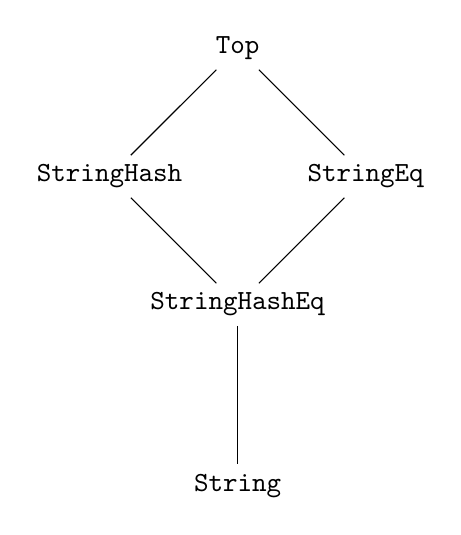
\begin{tikzpicture}[node distance=2.3cm]
    \node(Top) 												{\texttt{Top}};
    \node(StringEq)		[below right of=Top]			{\texttt{StringEq}};
    \node(StringHash)					[below left of=Top] 			{\texttt{StringHash}};
    \node(StringHashEq) [below left of=StringEq] {\texttt{StringHashEq}};
    \node(String) [below of=StringHashEq] {\texttt{String}};
    \draw(Top)      -- (StringEq);
    \draw(Top)      -- (StringHash);
    \draw(StringEq)      -- (StringHashEq);
    \draw(StringHash)      -- (StringHashEq);
    \draw(StringHashEq) -- (String);
  \end{tikzpicture}
  \caption{Operación \texttt{meet} entre \texttt{StringEq} y \texttt{StringHash}}
  \label{latticeInference}
\end{figure}

Consideremos el siguiente ejemplo, en donde se modifica una expresión de retorno del ejemplo \ref{ej2-4} con otro uso del parámetro \texttt{password}.

\begin{ej} \ \\
  \normalfont
  \label{ej2-9}
\begin{lstlisting}
  String<String login(String<String guess, String password) {
  	if (password.eq(guess)) return password.hash();
  	else return "Login failed";
  }
\end{lstlisting}
\end{ej}

Supongamos que \texttt{hash} retorna un \texttt{String}. Ahora se generan dos constraints sobre \texttt{password}, $\{\alpha <: [\mathtt{eq} : \mathtt{String<String} \rightarrow \mathtt{Bool<Bool}]\}$ y $\{\alpha <: [\mathtt{hash} : \mathtt{Unit<Unit} \rightarrow \mathtt{String<String}]\}$. El tipo $\alpha$ se resuelve con la operación \texttt{meet} entre ambos tipos de objeto, cuyo resultado $\mathtt{StringHashEq} \triangleq [\mathtt{eq} : \mathtt{String<String} \rightarrow \mathtt{Bool<Bool},\ \mathtt{hash} : \mathtt{Unit<Unit} \rightarrow \mathtt{String<String}]$ se muestra en la figura \ref{latticeInference}. El teorema \ref{teo1} muestra las reglas utilizadas para la aplicación de operaciones sobre la lattice.

\begin{teo} \label{teo1} \normalfont Si \texttt{x}, \texttt{y} y \texttt{z} pertenecen a una lattice de subtyping, se cumple lo siguiente: \\
  \begin{itemize}
    \item \texttt{x <: y}, \texttt{x <: z} $\implies$ \texttt{x <: y }$\wedge$\texttt{ z}
    \item \texttt{y <: x}, \texttt{z <: x} $\implies$ \texttt{y }$\vee$\texttt{ z <: x}
  \end{itemize}
\end{teo}
